\documentclass[12pt]{article}
\usepackage[a4paper,margin=1in]{geometry}
\usepackage{graphicx}
\usepackage{hyperref}
\usepackage{float}
\usepackage{caption}
\usepackage{listings}
\usepackage{xcolor}

\lstset{
  basicstyle=\ttfamily\footnotesize,
  backgroundcolor=\color{gray!5},
  frame=single,
  breaklines=true,
  postbreak=\mbox{\textcolor{red}{$\hookrightarrow$}\space},
  numbers=left,
  numberstyle=\tiny,
  xleftmargin=2em
}

\title{\textbf{Project 1 Report\\Multithreaded Banking Simulation}}
%\title{\textbf{ Multithreaded Banking Simulation}}
\author{Jack Vega \\ CSC 3502 — Operating Systems}
\date{\today}

\begin{document}
\maketitle

%%%%%%%%%%%%%%%%%%%%%%%%%%%%%%%%%%%%%%%%%
%				PHASE 1
%%%%%%%%%%%%%%%%%%%%%%%%%%%%%%%%%%%%%%%%%

%\newpage
\section{Phase 1}
\subsection{Objective}
The goal of Phase 1 was to design and implement a simple multithreaded banking simulation in \texttt{C} using the POSIX \texttt{pthread} library.
Each thread represents a bank teller performing multiple transactions on one or more shared accounts.

This phase focuses on building the basic concurrent framework, identifying race conditions, and applying synchronization mechanisms to ensure data integrity.

\subsection{Thread Design}
Each teller is represented by a thread executing the \texttt{teller\_thread()} function.
Every teller performs a fixed number of transactions (\texttt{TRANSACTIONS\_PER\_TELLER}) on a shared account array.

Each thread receives its unique teller ID as an argument to identify its log entries and printed output.

\subsection{Data Structures}
\begin{itemize}
  \item \textbf{Account:} contains an \texttt{account\_id}, \texttt{balance}, and \texttt{transaction\_count}.
  \item \textbf{logs:} a 2D array storing each thread’s transaction values for later verification.
\end{itemize}

\subsection{Correctness Verification}
At the end of execution:
\begin{enumerate}
  \item Each teller’s logged transactions are summed to compute the expected final balance.
  \item The expected balance is compared against the actual shared account balance after all threads complete.
\end{enumerate}

This allows us to evaluate whether a race condition occured or not.

\subsection{Challenges and Solutions}

\subsubsection{Correctness Verification}
At first, verifying correctness seemed quite challenging. However, after reflecting on how race conditions occur—specifically when multiple threads access the same memory location—I realized something important. Since arrays are inherently divided into distinct elements, as long as each thread writes to a unique index, a race condition cannot occur. This insight made it possible to safely log all thread operations and then aggregate their results in a single thread to verify the correctness of the final output.

\subsection{Performance Observations}
\begin{itemize}
  \item With only one account, there's little to no overhead
  \item Increasing the number of accounts (planned in later phases) will allow greater parallelism, but may present deadlock challenges.
  \item Although increasing the number of threads increases will speed up the throughput of data, it also increases the risk of race conditions.
\end{itemize}

\subsection{Program Output}
Example excerpt from a program run (10 threads, 10 transactions each):

\begin{lstlisting}[caption={Phase 1 Output}]
Initial Balance: $1000.00
Teller 1: Transaction 2
Thread 1: Depositing $100.000000
Thread 2: Depositing $100.000000
Teller 2: Transaction 0
...
Final Account Balances: $10900.00 <== Race Condition Detected!
Correct Account Balance: $11000.00
\end{lstlisting}

\subsection{Screenshots}
\begin{figure}[H]
  \centering
  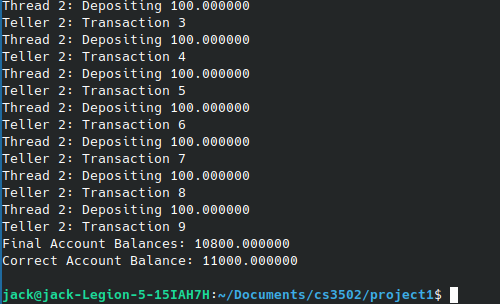
\includegraphics[width=0.8\textwidth]{phase1_race_cond.png}
  \caption{Phase 1 program output showing thread activity and final balance verification with a race condition having happened.}
\end{figure}

\subsection{Conclusion}
Phase 1 established a multithreaded structure for a banking simulation using POSIX threads showcasing race conditions.

%%%%%%%%%%%%%%%%%%%%%%%%%%%%%%%%%%%%%%%%%
%				PHASE 2
%%%%%%%%%%%%%%%%%%%%%%%%%%%%%%%%%%%%%%%%%

\newpage
\section{Phase 2}

\subsection{Objective}
The objective of Phase 2 was to perfect the multithreaded banking system from Phase 1 by introducing mutexes and preventing race conditions.
This phase also lays the groundwork for supporting multiple accounts.

\subsection{Key Differences from Phase 1}

Phase 2 builds directly on the Phase 1 foundation but introduces several structural and functional improvements:

\begin{itemize}
  \item \textbf{Dedicated \texttt{deposit()} Function:}
  All balance modifications are now handled through a separate function that encapsulates synchronization and overdraft checks.
  \item \textbf{Non-Blocking Locks:}
  Replaced \texttt{pthread\_mutex\_lock()} with \texttt{pthread\_mutex\_trylock()} to avoid stalling threads if an account is temporarily locked by another teller. (Stalling will be demonstrated in phase 3)
  \item \textbf{Transaction Retry Logic:}
  Threads reattempt failed transactions by decrementing the loop counter, ensuring each teller still completes the target number of successful transactions.
  \item \textbf{Enhanced Logging Structure:}
  The logs are now stored in a 3D array (\texttt{logs[account][teller][transaction]}) to properly record all teller activity per account. This is to further prepare for handling multiple accounts
  \item \textbf{Randomized Transaction Amounts:}
  Each transaction amount varies randomly, both positive (deposits) and negative (withdrawals), within a defined range.
\end{itemize}

\subsection{Approach}

Each teller thread repeatedly attempts to perform deposits or withdrawals on a randomly selected account.
If the account’s mutex cannot be acquired immediately, the thread pauses and waits until it is aquired.

\begin{itemize}
  \item \textbf{Thread Safety:}
  The shared account data remains protected by mutexes removing race conditions.
  \item \textbf{Validation:}
  Before modifying a balance, the system checks that withdrawals will not overdraft an account.
  Invalid operations are rejected.
  \item \textbf{Logging:}
  Each successful transaction is logged, allowing a “correct” final balance to be computed at the end for verification.
\end{itemize}

\subsection{Challenges and Solutions}
\paragraph{1. Overdraft Rejection.}
In earlier designs, withdrawing from a nearly empty account could cause negative balances.
By checking the condition \texttt{if (amount < 0 \&\& balance + amount < 0)}, we safely skip such operations and keep balances non-negative.

\subsection{Performance Observations}
\begin{itemize}
  \item \textbf{Overhead Trade-off:}
  Some CPU cycles are waiting, but this is offset by removing the possibility of race conditions.
\end{itemize}

\subsection{Program Output}

Example console output (abridged):

\begin{lstlisting}[caption={Phase 2 Output}]
Initial Balance: $1000.00
Thread 0: Depositing $63.22
Thread 0: Depositing $63.22
...
Thread 8: Withdrawing $100.31
Thread 8: Withdrawing $100.31
...

========================================
        Final Account Balances
========================================
Account 0: $393.11

========================================
        Correct Account Balances
========================================
Account 0: $393.11
\end{lstlisting}

The final reported balances match the computed “correct” balances, confirming that thread synchronization, validation logic worked properly, and no race conditions occured.

\subsection{Screenshots}
Include screenshots demonstrating:
\begin{itemize}
  \item The program running in a terminal showing concurrent deposits and withdrawals.
  \item The summary table of final and correct balances.
  \item A failed transaction example (where a lock could not be acquired).
\end{itemize}

\begin{figure}[H]
  \centering
  \includegraphics[width=0.8\textwidth]{phase2_output.png}
  \caption{Phase 2 output showing concurrent transactions and verified final balances.}
\end{figure}

\subsection{Conclusion}
Phase 2 introduced mutex's to the  banking simulation. This lets the program avoid race conditions and improves the accuracy of the account.

%%%%%%%%%%%%%%%%%%%%%%%%%%%%%%%%%%%%%%%%%
%				PHASE 3
%%%%%%%%%%%%%%%%%%%%%%%%%%%%%%%%%%%%%%%%%

\newpage
\section{Phase 3}

\subsection{Objective}
The objective of Phase 3 was to change the banking simulation to conduct balance transferes between accounts and explore the concept of deadlock occurrence.

\subsection{Design Overview}
Building upon Phase 2, this phase introduces two major system-level features:
\begin{itemize}
  \item \textbf{Inter-account Transfers:} Each teller now randomly selects two distinct accounts and transfers a random amount between them.
  \item \textbf{Deadlock Detection:} The system intentionally introduces potential circular wait conditions to observe a deadlock senario.
\end{itemize}

The introduction of multiple accounts makes synchronization significantly more complex. When two accounts are locked simultaneously for a transfer, threads risk entering a circular wait if they each hold one lock and wait for the other, this is called a deadlock.

\subsection{Deadlock Mechanism}
To simulate deadlocks intentionally, each transfer first locks the \texttt{from} account and then attempts to lock the \texttt{to} account.
A deliberate delay (\texttt{usleep(100)}) increases the likelihood that two threads will collide in opposite directions (e.g., A→B and B→A).

This demonstrates the occurrence of deadlocks.

\subsection{Thread Function Behavior}
Each teller thread:
\begin{enumerate}
  \item Randomly selects two distinct account IDs.
  \item Chooses a random transfer amount (between \$0.00 and \$125.94).
  \item Calls the \texttt{transfer()} function to perform the transaction.
\end{enumerate}

The randomness ensures diverse access patterns and increases contention probability.

\subsection{Program Output}
Example console output excerpt:
\begin{lstlisting}[caption={Phase 3 Output}]
Initial Balances:
    Account 0: $5000.00
    Account 1: $5000.00
Thread 0: Transferring $12.34 from account 0 to 1
Thread 1: Transferring $93.48 from account 1 to 0
... <== deadlocked

\end{lstlisting}

\subsection{Challenges and Solutions}
\paragraph{Deadlock Demonstration.}
The intentional \texttt{usleep()} delay combined with simultaneous locking of multiple accounts results in observable deadlocks.
This showcases how circular wait conditions arise when two threads attempt opposite transfers.

\paragraph{Transfer Consistency.}
Even under deadlock scenarios, accounts maintain valid balances due to the locking hierarchy ensuring no partial modifications occur.

\subsection{Screenshots}
\begin{figure}[H]
  \centering
  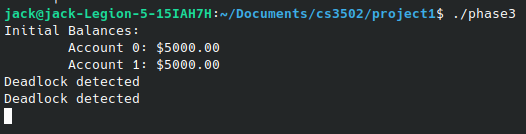
\includegraphics[width=0.8\textwidth]{phase3_deadlock.png}
  \caption{Phase 3 output showing a deadlock.}
\end{figure}

\subsection{Conclusion}
Phase 3 successfully demonstrates both inter-account transfer logic and the occurrence of deadlocks in concurrent systems.
This sets the foundation for \textbf{Phase 4}, where deadlock avoidance and recovery strategies will be introduced.

%%%%%%%%%%%%%%%%%%%%%%%%%%%%%%%%%%%%%%%%%
%				PHASE 4
%%%%%%%%%%%%%%%%%%%%%%%%%%%%%%%%%%%%%%%%%

\newpage
\section{Phase 4}

\subsection{Objective}
The objective of Phase 4 was to eliminate the deadlocks observed in Phase 3 by implementing an effective \textbf{deadlock avoidance mechanism}.
This was accomplished by applying a consistent \textbf{lock ordering policy}, ensuring that circular wait conditions cannot occur.

\subsection{Design Overview}
In previous phases, transfers between two accounts occasionally caused deadlocks when multiple threads attempted opposite transfers simultaneously (e.g., Account 0 → 1 and Account 1 → 0).
To resolve this, Phase 4 introduces the \texttt{safe\_transfer()} function, which orders all lock acquisitions by account ID, guaranteeing a globally consistent locking sequence.

\begin{itemize}
  \item \textbf{Lock Ordering:} Always lock the account with the smaller ID first.
  \item \textbf{Non-blocking Trylocks:} Use \texttt{pthread\_mutex\_trylock()} to gracefully handle contention without stalling.
  \item \textbf{Thread Retry:} Failed transactions are retried to ensure every teller still completes its designated number of operations.
\end{itemize}

This approach ensures that no two threads can hold locks in opposing orders, effectively preventing circular waits and deadlocks.

\subsection{Implementation Details}
The key innovation of Phase 4 lies in determining a global order for lock acquisition.
Given two accounts \texttt{from\_id} and \texttt{to\_id}, the system defines:
\begin{verbatim}
first  = min(from_id, to_id)
second = max(from_id, to_id)
\end{verbatim}
Threads then always lock the \texttt{first} account before the \texttt{second}, regardless of transfer direction.

This guarantees that no cyclic dependencies can form between threads, making deadlocks impossible by design.

\subsection{Program Output}
\begin{lstlisting}[caption={Phase 4 Output}]
Initial Balances:
....Account 0: $5000.00
....Account 1: $5000.00
Thread 2: Transferring $42.11 from account 0 to 1
Thread 4: Transferring $16.59 from account 1 to 0
Thread 7: Transferring $10.93 from account 0 to 1
...

Final Account Balances
....Account 0: $4988.38
....Account 1: $5011.62
\end{lstlisting}

No deadlocks occur even under high contention, confirming successful implementation of lock ordering.

\subsection{Challenges and Solutions}
\paragraph{1. Balancing Correctness and Concurrency.}
Initially, strict lock ordering slightly reduced concurrency since threads could not lock accounts in arbitrary order.
However, this trade-off was necessary to ensure total deadlock avoidance.

\paragraph{2. Retry Mechanism.}
The retry mechanism guarantees that failed transfers (due to temporarily busy accounts) are reattempted without affecting the total number of successful transactions per teller.

\subsection{Screenshots}
\begin{figure}[H]
  \centering
  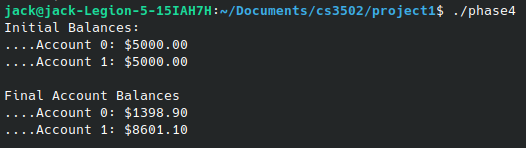
\includegraphics[width=0.8\textwidth]{phase4_completion.png}
  \caption{Phase 4 output showing no deadlocks or race conditions in the program output.}
\end{figure}

\subsection{Conclusion}
Phase 4 completes the core functionality of the multithreaded banking simulation by achieving both correctness and safety under concurrent inter-account transactions.
By applying a simple yet effective lock ordering rule, all deadlocks were eliminated without requiring complex detection or recovery systems.

This phase demonstrates the practical importance of structured synchronization design and forms the final step toward a fully reliable multithreaded banking model.

\end{document}
